%!TEX encoding = UTF-8 Unicode
\documentclass[french, a4paper, 12pt]{article}



%% Langue et compilation

\usepackage[utf8]{inputenc}
\usepackage[T1]{fontenc}
\usepackage[french]{babel}

%% LISTE DES PACKAGES

\usepackage{mathtools}     % package de base pour les maths
\usepackage{amsmath}       % mathematical type-setting
\usepackage{amssymb}       % symbols speciaux pour les maths
\usepackage{textcomp}      % symboles speciaux pour el text
\usepackage{gensymb}       % commandes generiques \degree etc...
\usepackage{tikz}          % package graphique
\usepackage{wrapfig}       % pour entourer a cote d'une figure
\usepackage{color}         % package des couleurs
\usepackage{xcolor}        % autre package pour les couleurs
\usepackage{pgfplots}      % pacakge pour creer des graph
\usepackage{epsfig}        % permet d'inclure des graph en .eps
\usepackage{graphicx}      % arguments dans includegraphics
\usepackage{pdfpages}      % permet d'insérer des pages pdf dans le document
\usepackage{subfig}        % permet de creer des sous-figure
\usepackage{pst-all}       % utile pour certaines figures en pstricks
\usepackage{lipsum}        % package qui permet de faire des essais
\usepackage{array}         % permet de faire des tableaux
\usepackage{multicol}      % plusieurs colonnes sur une page
\usepackage{enumitem}      % pro­vides user con­trol: enumerate, itemize and description
\usepackage{hyperref}      % permet de creer des hyperliens dans le document
\usepackage{lscape}        % permet de mettre une page en mode paysage
\usepackage{lmodern}       % permet d'avoir certains "fonts" de bonen qualite
\usepackage{fancyhdr}      % Permet de mettre des informations en hau et en bas de page      
\usepackage[framemethod=tikz]{mdframed} % breakable frames and coloured boxes
\usepackage[top=1.5cm, bottom=1.5cm, left=2.5cm, right=2.5cm]{geometry} % donne les marges
\usepackage[font=normalsize, labelfont=bf,labelsep=endash, figurename=Fig.]{caption} % permet de changer les legendes des figures
\usepackage{lewis}
\usepackage{bohr}
\usepackage{chemfig}
\usepackage{chemist}

%% LIBRAIRIES

\usetikzlibrary{plotmarks} % librairie pour les graphes
\usetikzlibrary{patterns}  % necessaire pour certaines choses predefinies sur tikz
\usetikzlibrary{shadows}   % ombres des encadres
\usetikzlibrary{backgrounds} % arriere plan des encadres


%% MISE EN PAGE

\pagestyle{fancy}     % Défini le style de la page

\renewcommand{\headrulewidth}{1pt}      % largeur du trait en haut de la page
\fancyhead[L]{Seconde générale}         % info coin haut gauche
\fancyhead[R]{Lycée Jean Guéhenno}  % info coin haut droit

% bas de la page
\renewcommand{\footrulewidth}{1pt}      % largeur du trait en bas de la page
\fancyfoot[L]{G. \bsc{LE DOUDIC}}  % info coin bas gauche
\fancyfoot[R]{TP 4 : Famille chimique}                         % info coin bas droit


\setlength{\columnseprule}{1pt} 
\setlength{\columnsep}{30pt}



%% NOUVELLES COMMANDES 

\DeclareMathOperator{\e}{e} % permet d'ecrire l'exponentielle usuellement


\newcommand{\gap}{\vspace{0.15cm}}   % defini une commande pour sauter des lignes
\renewcommand{\vec}{\overrightarrow} % permet d'avoir une fleche qui recouvre tout le vecteur
\newcommand{\bi}{\begin{itemize}}    % begin itemize
\newcommand{\ei}{\end{itemize}}      % end itemize
\newcommand{\bc}{\begin{center}}     % begin center
\newcommand{\ec}{\end{center}}       % end center
\newcommand\opacity{1}               % opacity 
\pgfsetfillopacity{\opacity}

\newcommand*\Laplace{\mathop{}\!\mathbin\bigtriangleup} % symbole de Laplace

\frenchbsetup{StandardItemLabels=true} % je ne sais plus

\newcommand{\smallO}[1]{\ensuremath{\mathop{}\mathopen{}o\mathopen{}\left(#1\right)}} % petit o

\newcommand{\cit}{\color{blue}\cite} % permet d'avoir les citations de couleur bleues
\newcommand{\bib}{\color{black}\bibitem} % paragraphe biblio en noir et blanc
\newcommand{\bthebiblio}{\color{black} \begin{thebibliography}} % idem necessaire sinon bug a cause de la couleur
\newcommand{\ethebiblio}{\color{black} \end{thebibliography}}   % idem
%%% TIKZ


%% COULEURS 


\definecolor{definitionf}{RGB}{220,252,220}
\definecolor{definitionl}{RGB}{39,123,69}
\definecolor{definitiono}{RGB}{72,148,101}

\definecolor{propositionf}{RGB}{255,216,218}
\definecolor{propositionl}{RGB}{38,38,38}
\definecolor{propositiono}{RGB}{109,109,109}

\definecolor{theof}{RGB}{255,216,218}
\definecolor{theol}{RGB}{160,0,4}
\definecolor{theoo}{RGB}{221,65,100}

\definecolor{avertl}{RGB}{163,92,0}
\definecolor{averto}{RGB}{255,144,0}

\definecolor{histf}{RGB}{241,238,193}

\definecolor{metf}{RGB}{220,230,240}
\definecolor{metl}{RGB}{56,110,165}
\definecolor{meto}{RGB}{109,109,109}


\definecolor{remf}{RGB}{230,240,250}
\definecolor{remo}{RGB}{150,150,150}

\definecolor{exef}{RGB}{240,240,240}

\definecolor{protf}{RGB}{247,228,255}
\definecolor{protl}{RGB}{105,0,203}
\definecolor{proto}{RGB}{174,88,255}

\definecolor{grid}{RGB}{180,180,180}

\definecolor{titref}{RGB}{230,230,230}

\definecolor{vert}{RGB}{23,200,23}

\definecolor{violet}{RGB}{180,0,200}

\definecolor{copper}{RGB}{217, 144, 88}

%% Couleur des ref

\hypersetup{
	colorlinks=true,
	linkcolor=black,
	citecolor=blue,
	urlcolor=black
		   }

%% CADRES


% %%%%%%%%%% DEFINITION
% \newmdenv[tikzsetting={fill=definitionf}, linewidth=2pt, linecolor=definitionl, outerlinewidth=0pt, innertopmargin=5pt, innerbottommargin=5pt, innerleftmargin=5pt, innerrightmargin=5pt, leftmargin=0pt]{definition}

% \newmdenv[ tikzsetting={drop shadow={ shadow xshift=1ex, shadow yshift=-0.5em, fill=definitiono, opacity=1, every shadow } }, outerlinewidth=2pt, outerlinecolor=white, linecolor=white, innertopmargin=0pt, innerbottommargin=0pt, innerleftmargin=0pt, innerrightmargin=0pt]{ombredef}


% %%%%%%%%%% THEOREME

% \newmdenv[tikzsetting={fill=theof}, linewidth=2pt, linecolor=theol, outerlinewidth=0pt, innertopmargin=5pt, innerbottommargin=5pt, innerleftmargin=5pt, innerrightmargin=5pt, leftmargin=0pt]{theo}

% \newmdenv[ tikzsetting={drop shadow={ shadow xshift=1ex, shadow yshift=-0.5em, fill=theoo, opacity=1, every shadow } }, outerlinewidth=2pt, outerlinecolor=white, linecolor=white, innertopmargin=0pt, innerbottommargin=0pt, innerleftmargin=0pt, innerrightmargin=0pt]{ombretheo}


% %%%%%%%%%% METHODE

% \newmdenv[tikzsetting={fill=metf}, linewidth=2pt, linecolor=metl, outerlinewidth=0pt, innertopmargin=5pt, innerbottommargin=5pt, innerleftmargin=5pt, innerrightmargin=5pt, leftmargin=0pt]{met}

% \newmdenv[ tikzsetting={drop shadow={ shadow xshift=1ex, shadow yshift=-0.5em, fill=meto, opacity=1, every shadow } }, outerlinewidth=2pt, outerlinecolor=white, linecolor=white, innertopmargin=0pt, innerbottommargin=0pt, innerleftmargin=0pt, innerrightmargin=0pt]{ombremet}



%%%%%%%%%%% RQ

\newmdenv[tikzsetting={fill=remf}, linewidth=2pt, linecolor=remf, outerlinewidth=0pt, innertopmargin=5pt, innerbottommargin=5pt, innerleftmargin=5pt, innerrightmargin=5pt, leftmargin=0pt]{remarque}

\newmdenv[ tikzsetting={drop shadow={ shadow xshift=1ex, shadow yshift=-0.5em, fill=remo, opacity=1, every shadow } }, outerlinewidth=2pt, outerlinecolor=white, linecolor=white, innertopmargin=0pt, innerbottommargin=0pt, innerleftmargin=0pt, innerrightmargin=0pt]{ombreremarque}

%%%%%%%%%%% Cadre pour le titre

\tikzset{every shadow/.style={opacity=1}}

\global\mdfdefinestyle{doc}{backgroundcolor=white, shadow=true, shadowcolor=propositiono, linewidth=1pt, linecolor=black, shadowsize=5pt}
\global\mdfdefinestyle{titr}{backgroundcolor=metf, shadow=true, shadowcolor=propositiono, linewidth=1pt, linecolor=black, shadowsize=5pt}
\global\mdfdefinestyle{theo}{backgroundcolor=theof, shadow=true, shadowcolor=theoo, linewidth=1pt, linecolor=theol, shadowsize=5pt}
\global\mdfdefinestyle{prop}{backgroundcolor=theof, shadow=true, shadowcolor=propositiono, linewidth=1pt, linecolor=theol, shadowsize=5pt}
\global\mdfdefinestyle{def}{backgroundcolor=definitionf, shadow=true, shadowcolor=definitiono, linewidth=1pt, linecolor=definitionl, shadowsize=5pt}
\global\mdfdefinestyle{histo}{backgroundcolor=histf, shadow=true, shadowcolor=propositiono, linewidth=1pt, linecolor=black, shadowsize=5pt}
\global\mdfdefinestyle{avert}{backgroundcolor=white, shadow=true, shadowcolor=averto, linewidth=1pt, linecolor=avertl, shadowsize=5pt}
\global\mdfdefinestyle{met}{backgroundcolor=metf, shadow=true, shadowcolor=meto, linewidth=1pt, linecolor=metl, shadowsize=5pt}
\global\mdfdefinestyle{rem}{backgroundcolor=metf, shadow=true, shadowcolor=meto, linewidth=1pt, linecolor=metf, shadowsize=5pt}
\global\mdfdefinestyle{exo}{backgroundcolor=exef, shadow=true, shadowcolor=propositiono, linewidth=1pt, linecolor=exef, shadowsize=5pt}
\global\mdfdefinestyle{not}{backgroundcolor=definitionf, shadow=true, shadowcolor=propositiono, linewidth=1pt, linecolor=black, shadowsize=5pt}
\global\mdfdefinestyle{proto}{backgroundcolor=protf, shadow=true, shadowcolor=proto, linewidth=1pt, linecolor=protl, shadowsize=5pt}

%%%%%%
\definecolor{cobalt}{rgb}{0.0, 0.28, 0.67}
\definecolor{applegreen}{rgb}{0.55, 0.71, 0.0}

\usepackage{tcolorbox}
  \tcbuselibrary{most}
  \tcbset{colback=cobalt!5!white,colframe=cobalt!75!black}



\newtcolorbox{definition}[1]{
	colback=applegreen!5!white,
  	colframe=applegreen!65!black,
	fonttitle=\bfseries,
  	title={#1}}
\newtcolorbox{Programme}[1]{
	colback=cobalt!5!white,
  	colframe=cobalt!65!black,
	fonttitle=\bfseries,
  	title={#1}}  

\newtcolorbox{Exercice}[1]{
  colback=cobalt!5!white,
  colframe=cobalt!65!black,
  fonttitle=\bfseries,
  title={#1}}  

  \newtcolorbox{Protocol}[1]{
  colback=cyan!5!white,
  colframe=cyan!65!black,
  fonttitle=\bfseries,
  title={#1}}  

\newtcolorbox{Resultat}[1]{
	colback=theof,%!5!white,
	colframe=theoo!85!black,
  fonttitle=\bfseries,
	title={#1}} 	


\def\width{12}
\def\hauteur{5}

\setlength{\parskip}{0pt}%
\setlength{\parindent}{18pt}


%% MODIFICATION DE CHAPTER  
\makeatletter
\def\@makechapterhead#1{%
  %%%%\vspace*{50\p@}% %%% removed!
  {\parindent \z@ \raggedright \normalfont
    \ifnum \c@secnumdepth >\m@ne
        \huge\bfseries \@chapapp\space \thechapter
        \par\nobreak
        \vskip 20\p@
    \fi
    \interlinepenalty\@M
    \Huge \bfseries #1\par\nobreak
    \vskip 40\p@
  }}
\def\@makeschapterhead#1{%
  %%%%%\vspace*{50\p@}% %%% removed!
  {\parindent \z@ \raggedright
    \normalfont
    \interlinepenalty\@M
    \Huge \bfseries  #1\par\nobreak
    \vskip 40\p@
  }}
  
  \newcommand{\isotope}[3]{%
     \settowidth\@tempdimb{\ensuremath{\scriptstyle#1}}%
     \settowidth\@tempdimc{\ensuremath{\scriptstyle#2}}%
     \ifnum\@tempdimb>\@tempdimc%
         \setlength{\@tempdima}{\@tempdimb}%
     \else%
         \setlength{\@tempdima}{\@tempdimc}%
     \fi%
    \begingroup%
    \ensuremath{^{\makebox[\@tempdima][r]{\ensuremath{\scriptstyle#1}}}_{\makebox[\@tempdima][r]{\ensuremath{\scriptstyle#2}}}\text{#3}}%
    \endgroup%
  }%

\makeatother


%%
%% DEBUT DU DOCUMENT
%%
\begin{document}


%%%%%%
\tikzset{every shadow/.style={opacity=1}}

\global\mdfdefinestyle{doc}{backgroundcolor=white, shadow=true, shadowcolor=propositiono, linewidth=1pt, linecolor=black, shadowsize=5pt}
\global\mdfdefinestyle{titr}{backgroundcolor=titref, shadow=true, shadowcolor=propositiono, linewidth=1pt, linecolor=black, shadowsize=5pt}
\global\mdfdefinestyle{theo}{backgroundcolor=theof, shadow=true, shadowcolor=theoo, linewidth=1pt, linecolor=theol, shadowsize=5pt}
\global\mdfdefinestyle{prop}{backgroundcolor=theof, shadow=true, shadowcolor=propositiono, linewidth=1pt, linecolor=theol, shadowsize=5pt}
\global\mdfdefinestyle{def}{backgroundcolor=definitionf, shadow=true, shadowcolor=definitiono, linewidth=1pt, linecolor=definitionl, shadowsize=5pt}
\global\mdfdefinestyle{histo}{backgroundcolor=histf, shadow=true, shadowcolor=propositiono, linewidth=1pt, linecolor=black, shadowsize=5pt}
\global\mdfdefinestyle{avert}{backgroundcolor=white, shadow=true, shadowcolor=averto, linewidth=1pt, linecolor=avertl, shadowsize=5pt}
\global\mdfdefinestyle{met}{backgroundcolor=metf, shadow=true, shadowcolor=meto, linewidth=1pt, linecolor=metl, shadowsize=5pt}
\global\mdfdefinestyle{rem}{backgroundcolor=metf, shadow=true, shadowcolor=meto, linewidth=1pt, linecolor=metf, shadowsize=5pt}
\global\mdfdefinestyle{exo}{backgroundcolor=exef, shadow=true, shadowcolor=propositiono, linewidth=1pt, linecolor=exef, shadowsize=5pt}
\global\mdfdefinestyle{not}{backgroundcolor=definitionf, shadow=true, shadowcolor=propositiono, linewidth=1pt, linecolor=black, shadowsize=5pt}
\global\mdfdefinestyle{proto}{backgroundcolor=protf, shadow=true, shadowcolor=proto, linewidth=1pt, linecolor=protl, shadowsize=5pt}
\begin{center}
	\begin{mdframed}[style=titr, leftmargin=15pt, rightmargin=15pt, innertopmargin=8pt, innerbottommargin=8pt, innerrightmargin=10pt, innerleftmargin=10pt]
		
		
		\begin{center}
			\Large{\textbf{Chapitre 5 : Les circuits électriques et les capteurs}} \\
			% \large{\textbf{TP8: \og{} Bien choisir son eau\fg{}  et TP8: \og{}  Les molécules \fg{}}}
		\end{center}
	\end{mdframed}
\end{center}
\bigskip

\doc{1}{Bulletin officiel}{
\begin{center}
	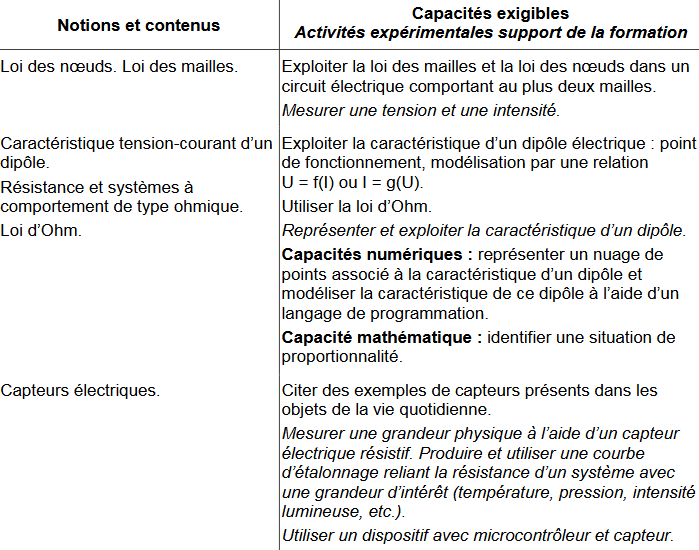
\includegraphics[width=.8\textwidth]{Bo.png}
\end{center}
}


\doc{2}{Exercices dans le livre scolaire}{
		\begin{enumerate}
			\item Reconnaître des n\oe uds et des mailles : exercices 4, 6 page 313.
			\item Lois de Kirchoff : exercices 7, 8, 9 page 313.
			\item Modélisation de la caractéristique d'un dipôle : exercice 18 page 316.
			% \item Le modèle de Lewis : exercices 9, 15, 16 p 116.
		\end{enumerate}
}
	\noindent \textbf{Quiz sur les circuits électriques et les capteurs}

	\begin{minipage}{.2\textwidth}
		\centering
		
\includegraphics[width=1\textwidth]{Quiz1.png}
		\protect Quiz 1 - Les circuits électriques : \url{https://forms.office.com/r/rLk3haXCTN}
	\end{minipage}\hfill
	\begin{minipage}{.3\textwidth}
		\centering
		
\includegraphics[width=.7\textwidth]{Quiz2.png}

		Quiz 2 - Les lois de Kirchhoff : \url{https://forms.office.com/r/JWeK6W4iiY?origin=lprLink}
	\end{minipage}\hfill
	\begin{minipage}{.3\textwidth}
		\centering
		
\includegraphics[width=.7\textwidth]{Quiz3.png}

		Quiz 3 : La caractéristique d'un dipôle : \hfill \url{https://forms.office.com/r/7vP0pmcU7Z}
	\end{minipage}
% \begin{figure}[ht]
% 	% \centering
% 	\subfloat[Quiz 1 - Les circuits électriques : \hfill \url{https://forms.office.com/r/rLk3haXCTN}]{
\includegraphics[width=.2\textwidth]{Quiz1.png}}\hfill
% 	\subfloat[Quiz 2 - Les lois de Kirchoff : \hfill \url{https://forms.office.com/r/JWeK6W4iiY?origin=lprLink}]{
\includegraphics[width=.2\textwidth]{Quiz2.png}}\hfill
% 	\subfloat[Quiz 3 : La caractéristique d'un dipôle : \hfill \url{https://forms.office.com/r/7vP0pmcU7Z}]{
\includegraphics[width=.2\textwidth]{Quiz3.png}}\hfill
% 	% \subfloat[Pour aller plus loin : \hfill \url{https://learningapps.org/view23412425}]{
\includegraphics[width=.2\textwidth]{PourAllerPLusLoin.png}}\hfill

% % \end{figure}

\clearpage
% \section*{Introduction}


\section{À la découverte des circuits électriques : intensité et tension électrique}
\begin{center}
	\textit{ref : Le livre scolaire page 308-310}
\end{center}
L'électricité est le nom que l'on donne au phénomène physique qui rend possible l'utilisation de tous nos appareils du quotidien. Deux grandeurs physiques majeures sont à prendre en compte pour tout montage électrique: la tension et l'intensité. Savoir les mesurer, les calculer, les assembler et les dissocier permet de maitriser les montages électriques.\medskip

Ce cours introduit dans un premier temps, des généralités sur les circuits électriques, pour ensuite s'intéresser à l'intensité puis à la tension. Pour finalement décrire le lien mathématique qui les lie.

\subsection{Deux types de circuits électriques}



L'électricité est créee par un mouvement porteur de charges (électrons) dans un circuit électrique. Un circuit électrique est une association de dipôles reliés entre les autres par des fils électriques. L'un de ces dipôles est un générateur qui délivre le courant électrique. les autres dipôles seront considérés comme des récepteurs. 

\begin{definition}{Définition 1 - Dipôle électrique}
	Un dipôle électrique est un élément d'un circuit électrique possédant deux bornes.
\end{definition}


On distingue deux types de circuits électriques : 
\begin{enumerate}
	\item Les circuits en \textbf{série} qui ne comportent qu'une seule maille.
	\item Les circuits en \textbf{dérivation} qui comportent au moins deux mailles.
\end{enumerate}

La portion de circuit entre deux n\oe uds consécutifs constitue une \textbf{branche} du circuit. La branche qui contient le générateur est appelée la branche \textbf{principale} , et les autres branches étant les branches \textbf{dérivées}.\medskip 

\begin{minipage}[l]{.47\textwidth}
\doc{1}{Un circuit électriques à plusieurs mailles}{
	\centering
\begin{circuitikz}
	\draw (-.3,2.1) node{+};
	\draw (-.3,0.9) node{-};
	
	\draw[thick] (0,0) to[rmeter, t=G, v^>=\textcolor{red}{$u$}] (0,3);
	\draw[thick] (0,3) -- (3,3);
	\draw[thick] (3,3) to [lamp] (3,0);
	\draw[thick] (3,0) -- (0,0);
	\draw[thick] (0+3,3) -- (3+3,3);
	\draw[thick] (3+3,3) to [R] (3+3,0);
	\draw[thick] (3+3,0) -- (0+3,0);
\end{circuitikz}


\textit{Ce circuit comprend une pile qui est le générateur qui fournit l'électricité dans le circuit, une lampe et une résistance R.}
}
\end{minipage}\hfill
\begin{minipage}[r]{.46\textwidth}
	\centering
	\exo{1}{Indiquer sur le \bsc{Document 1} : }{
\begin{itemize}
	\item en rouge la branche principale et avec des couleurs différentes les branches secondaires;
	\item Indiquer les noeuds sur le circuit à l'aide d'un $\bullet$;
	\item Noter avec la lettre R la résistance et la lampe avec la lettre L. 
\end{itemize}
}
\end{minipage}
\medskip

\begin{definition}{Définition 2 - Un n\oe ud}
	Un n\oe ud est l'intersection entre au moins 3 fils électriques.
\end{definition}
\medskip

\begin{definition}{Définition 3 - Une maille}
	C'est un chemin fermé, ne comportant pas forcément de générateur.
\end{definition}

\clearpage
\subsection{Le courant électrique}

Le courant électrique circule à l'extérieur du générateur depuis la borne positive vers la borne négative : \textbf{c'est le sens conventionnel} du courant électrique. On représente le sens du courant électrique par une flèche (\textcolor{red}{rouge} quand c'est possible) comme sur le \bsc{document 2}.\medskip

\begin{definition}{Définition 4 - L'intensité du courant}
	L'intensité du courant est une grandeur quantifiant le nombre d'électrons qui traversent un fil ou un dipôle en une seconde.\medskip
	
	Elle est notée $I$ et s'exprime en ampère, noté A.
	
\end{definition}




\begin{Proposition}{Propriété 1 - L'intensité du courant électrique}
	Dans un circuit \textbf{en série}, l'intensité du courant électrique est la même en tout point du circuit. De même l'intensité du courant qui entre dans un dipôle est toujours égale à l'intensité qui en ressort.
\end{Proposition}

% \clearpage
\subsection{La tension du courant}


\begin{definition}{Definition 5 - La tension électrique}

 La tension électrique est une grandeur caractérisant une différence d'état électrique entre deux points d'un circuit.\medskip

La tension noté $U$ s'exprime en volts notés V.
	
\end{definition}

La tension électrique aux bornes d'un dipôle, notée $U$, est représentée par une flèche qui pointe vers la première lettre de sa notaion symbolique comme par exemple sur le \bsc{Document 2} la flèche représentant la tension entre les bornes C et D notée $U_{CD}$ est dirigée vers le point C.\medskip



\begin{Proposition}{Propriété 2 - La tension électrique aux bornes d'un dipôle}

	La tension aux bornes de dipôles associés en dérivation est la même.
\end{Proposition}

\doc{3}{La tension électrique dans un circuit électrique}{
\centering
\begin{circuitikz}
	
	\ctikzset{voltage shift=2}
	\draw[thick] (-.3,2.1) node{+};
	\draw (-.3,0.9) node{-};
	
	\draw[thick] (0,0) to[rmeter, t=G, v^>=\textcolor{red}{$u$},i^>=\textcolor{red}{$i_1$}] (0,3);
	\draw[thick] (0,3) to[rmeter, t= A, i^>=\textcolor{red}{$i_1$}] (3,3);
	\draw (1.5,3.8) node{Ampèremètre};
	\draw[thick] (3,3) to [lamp, i^>=\textcolor{red}{$i_2$}] (3,0);
	\draw[thick] (3,0) -- (0,0);
	\draw[thick] (3,3) to [lamp, i>^=\textcolor{red}{$i_2$}] (3,0);
	\draw[thick] (3,0) -- (0,0);
	\draw[thick] (0+2,3) -- (3+3,3);
	\draw[thick] (3+2,3) to [R, v^=$U_{CD}$,i^>=\textcolor{red}{$i_3$}] (3+2,0);
	\draw[thick] (6,3) -- (7,3) to[rmeter, t = V] (7,0) -- (5,0);
	\draw[thick] (3+2,3) to [R,i>^=\textcolor{red}{$i_3$}] (3+2,0);
	\draw[thick] (3+2,0) -- (0+3,0);
	\draw (8,1.5) node[rotate = 90]{Voltmètre};
	\draw (0,3) node{$\bullet$};
	\draw (0,3.3) node{A};
	\draw (3,3) node{$\bullet$};
	\draw (3,3.3) node{B};
	\draw (5,3) node{$\bullet$};
	\draw (5,3.3) node{C};
	\draw (5,0) node{$\bullet$};
	\draw (5,-0.3) node{D};
	\draw (3,0) node{$\bullet$};
	\draw (3,-0.3) node{E};
	\draw (0,0) node{$\bullet$};
	\draw (0,-0.3) node{F};
\end{circuitikz}

\textit{Dans ce circuit on a branché un \textbf{voltmètre} pour mesurer la tension $U_{CD}$ et on a branché un \textbf{ampèremètre} pour mesurer le courant $i_1$. Un ampèremètre est toujours branché en \textbf{série} tandis qu'un voltmètre est toujours branché en \textbf{dérivation}.}

}
\clearpage
\section{Les lois décrivant les circuits électriques : la loi des noeuds et la loi des mailles}
\begin{center}
	\textit{ref : Le livre scolaire page 308-310}
\end{center}

\subsection{La loi des n\oe uds}
La quantité d'électrons qui circulent dans le circuit se conserve. La loi des n\oe uds traduit cette conservation : En chaque n\oe ud le courant se divise en parties qui peuvent être égales ou non.

\begin{definition}{Loi 1 - La loi des n\oe uds}
	La somme des intensités des courants électriques qui arrivent à un n\oe ud est égale à la somme des intensités qui en repartent.
	\begin{equation}
		i_1= i_2 +i_3
	\end{equation}
\end{definition}

\exo{2}{Application de la loi des n\oe uds}{

Dans le circuit du \bsc{documemt 3}, on a mesuré $i_3 = 0,5~\rm A$ et $i_2=0,2~\rm A$. Calculez la valeur de $i_1$.\medskip

\textbf{Solution :} D'après la loi des n\oe uds $i_1 = i_2 + i_3$. Donc $i_1 = 0.7~\rm A$.
% \dotfill \medskip

% \dotfill

}
% \clearpage
\subsection{Les conventions d'orientation et la loi des mailles}

\subsubsection{Les conventions d'orientation}
Les intensités de courant et les tensions électriques sont des grandeurs algébriques (elles peuvent être positives ou négatives). C'est pourquoi on adopte des conventions de notations et de branchement\medskip

\begin{minipage}{.6\textwidth}
\begin{itemize}
	\item Pour les générateurs : 
	\begin{enumerate}
		\item L'intensité du courant électrique I est représenté par une flèche \og{}sortant\fg{} de la borne positive du générateur.
		\item La tension U aux bornes d'un générateur est représentée par une flèche au-dessus du symbole, dans le même sens que le courant.
	\end{enumerate}

	\item Pour les récepteurs : les flèches tension et courant sont orientées dans des sens opposés
\end{itemize}
\end{minipage}\hfill
\begin{minipage}{.3\textwidth}
	\centering
	\begin{circuitikz}
		\draw[thick] (0,0) to[rmeter, t= G, v^>=$U_G$, i^>=$i$] (2,0);
		\draw (1.5,0.3) node{+};
	\end{circuitikz}
	\captionof{figure}{Convention pour un générateur}\vspace{1cm}

	\begin{circuitikz}
		\draw[thick] (0,0) to [R, i>^=$i$,v=$U_R$] (2,0);
	\end{circuitikz}
	\captionof{figure}{Convention pour un récepteur}
\end{minipage}

\subsubsection{La loi des mailles}
\medskip

\begin{definition}{Loi 2 - la loi des mailles}
	\medskip
	La somme algébrique des tensions des dipôles le long d'une maille est égale à 0V. 
\end{definition}\medskip

\begin{minipage}{.4\textwidth}
Pour additionner les tensions dans la maille orientée, on commence par orienter arbitrairement la maille et on affecte : 
\begin{enumerate}
	\item un signe \og{}+\fg{} à une tension si sa flèche est dans le même sens que celui du parcours;
	\item un signe \og{}-\fg{} dans le cas contraire.
\end{enumerate}

Lorsqu'on applique la \textbf{loi des mailles} a la maille ABCDA du circuit représenté sur la figure 5. On obtient l'équations suivante :
\begin{equation}
	-U_G+U_2+U_1=0
\end{equation}
\end{minipage}\hfill
\begin{minipage}{.5\textwidth}
	\centering
\begin{circuitikz}[
	line width = 0.8pt,
	voltage shift = 0.5]
	\draw (0,0)     to[rmeter, t=G, v>=\textcolor{red}{$U_G$},i^>=\textcolor{red}{$i_1$}]  (0, 4) -- ++ (0.5,0) 
					to[R,v=$U_1$,i^>=\textcolor{red}{$i_1$}]      ++  (2, 0) -- ++ (0.5,0) -- ++  (0,-1)
					to[R,v=$U_2$,i^>=\textcolor{red}{$i_1$}]      ++  (0,-2) -- ++ (0 ,-1) 
					to[short] (0,0);
	\draw (0,4) node{$\bullet$};
	\draw (0,4.3) node{A};
	\draw (3,4) node{$\bullet$};
	\draw (3,4.3) node{B};
	\draw (3,0) node{$\bullet$};
	\draw (3,-0.3) node{C};
	\draw (0,0) node{$\bullet$};
	\draw (0,-0.3) node{D};
	\draw[thick] (-.3,2.7) node{+};
	\draw (-.3,1.2) node{-};
	\draw[thick, cyan,-|>] (1.5,1.5) arc (-230:20:.5);
	\end{circuitikz}
	\captionof{figure}{L'unique maille de ce circuit est orientée dans le sens trigonométrique (anti-horaire).}
\end{minipage}



\exo{3}{Application de la loi des mailles à un circuit électrique}{

On a représenté ci-dessous un circuit qui comporte trois mailles. Il comporte un générateur de tension, trois résistances ($R_1, R_2$ et $R_3$, ainsi qu'une diode électroluminescente ou LED). Avec l'aide de ce circuit vous devrez répondre aux questions suivantes: 


\begin{enumerate}
	\item Orientez les trois mailles que comporte ce circuit.
	\item Écrivez la loi des mailles pour chacune des trois mailles. 
	\item Sachant que la tension délivrée par le générateur vaut $U_G = 5V$ et que $U_1 = 2V$, en déduire la valeur de la tension aux bornes de la résistance $R_2$ notée $U_2$. 
\end{enumerate}
\noindent\textbf{Répondez aux questions ci-dessous:}

\begin{minipage}{.45\textwidth}
\begin{circuitikz}[
	line width = 0.8pt,
	voltage shift = 0.5]
	\draw (0,0)     to[rmeter, t=G, v>=\textcolor{red}{$U_G$},i^>=\textcolor{red}{$i_1$}]  (0, 4) -- ++ (0.5,0) 
					to[R,v=$U_1$,i^>=\textcolor{red}{$i_1$}]      ++  (2, 0) -- ++ (0.5,0) coordinate (aux)
												   -- ++  (0,-1)
					to[R,v=$U_2$,i^>=\textcolor{red}{$i_2$}]      ++  (0,-2) -- ++ (0 ,-1) 
		  (aux)     to[short]           ++  (2, 0)
					to[R,v=$U_3$,i^>=\textcolor{red}{$i_3$}]      ++  (0,-4) -- ++ (-0.5,0)
					to [diode,v=$U_4$]      ++  (-1,0) -- (0,0);% coordinate (aux)
					% to[short] (0,0);
					\draw (0,0)     to[rmeter, t=G, v>=\textcolor{red}{$U_G$},i^>=\textcolor{red}{$i_1$}]  (0, 4) -- ++ (0.5,0) 
					to[R,v=$U_1$,i>^=\textcolor{red}{$i_1$}]      ++  (2, 0) -- ++ (0.5,0) coordinate (aux)
												   -- ++  (0,-1)
					to[R,v=$U_2$,i>^=\textcolor{red}{$i_2$}]      ++  (0,-2) -- ++ (0 ,-1) 
		  (aux)     to[short]           ++  (2, 0)
					to[R,v=$U_3$,i>^=\textcolor{red}{$i_3$}]      ++  (0,-4) -- ++ (-0.5,0)
					to [diode,v=$U_4$]      ++  (-1,0) -- (0,0);% coordinate (aux)
					%to[short] (0,0);
	\draw (0,4) node{$\bullet$};
	\draw (0,4.3) node{A};
	\draw (3,4) node{$\bullet$};
	\draw (3,4.3) node{B};
	\draw (5,4) node{$\bullet$};
	\draw (5,4.3) node{C};
	\draw (5,0) node{$\bullet$};
	\draw (5,-0.3) node{D};
	\draw (3,0) node{$\bullet$};
	\draw (3,-0.3) node{E};
	\draw (0,0) node{$\bullet$};
	\draw (0,-0.3) node{F};
	\draw[thick] (-.3,2.7) node{+};
	\draw (-.3,1.2) node{-};
	
	\end{circuitikz}
\end{minipage}
\begin{minipage}{.5\textwidth}
	\noindent 2. Lois des mailles
	\begin{itemize}
		\item Maille ABCDFA : $-U_G+U_1+U_3+U_4 = 0~\rm V$
		\item Maille ABEFA  : $-U_G+U_1+U_2 = 0~\rm V$
		\item Maille BCDEB  : $-U_2+U_3+U_4 = 0~\rm V$
	\end{itemize}
	\noindent 3. Calcul de $U_2$ : 

	D'après la maille ABEFA, il vient : $U_2=U_G-U_1$ et l'application numérique donne $U_2 = 3~\rm V$.

	
\end{minipage}
% \vspace{3cm}

}

\clearpage

\section{Les caractéristiques d'un dipôle et son point de fonctionnement}
\begin{center}
	\textit{ref : Le livre scolaire page 308-310}
\end{center}
\subsection{Comment peut-on caractériser un dipôle électrique ?}

Pour mieux connaître un dipôle, on peut le soumettre à différentes sollicitations. Par exemple pour caractériser un générateur ou une résistance on peut mesurer la tension à leurs bornes et le courant électrique qui les traverse à l'aide d'un voltmètre et d'un ampèremètre.

La caractéristique d'un dipôle est basée sur l'ensemble des couples de valeurs mesurées (I et U).

\begin{definition}{Définition 6 - Caractéristique tension - courant et courant - tension d'un dipôle}
	
	\textbf{La caractéristique tension-courant} d'un dipôle est la représentation graphique de l'évolution de sa tension $U$ en fonction de l'intensité $I$ du courant électrique qui le traverse. Autrement dit c'est la courbe d'équation : 
	\begin{equation}
		U = f(I).
	\end{equation}

	\textbf{La caractéristique tension-courant} d'un dipôle est la représentation graphique de l'évolution de l'intensité du courant électrique $I$ en fonction de la tension $U$ qui le traverse. Autrement dit c'est la courbe d'équation : 
	\begin{equation}
		I = g(U).
	\end{equation}
\end{definition}

\subsection{Caractéristique d'un conducteur ohmique : La loi d'Ohm}

pour déterminer la caractéristique d'un conducteur ohmique, c'est à dire une résistance $R$. On doit la brancher sur un générateur de courant qui va délivrer un courant électrique d'intensité $I$ à la résistance. On mesure ce courant à l'aide d'un ampèremetre. Aux bornes de la résistance, en dérivation, on branche un voltmètre pour mesurer la tension $U$ aux bornes de la résistance. De cette façon, on peut mesurer la tension U en fonction du courant I qui traverse la résistance.\medskip


\begin{minipage}{.35\textwidth}
	\centering
	\begin{circuitikz}[
		line width = 0.8pt,
		voltage shift = 0.5]
		\draw (0,0)     to[rmeter, t=G, v>=\textcolor{red}{$U_G$},i^>=\textcolor{red}{$i_1$}]  (0, 4) -- ++ (3,0) -- ++  (0,-1)
						to[R,v=$U_1$,i^>=\textcolor{red}{$i_1$}]      ++  (0,-2) -- ++ (0,-1) -- ++ (-3,0);
	\end{circuitikz}
\end{minipage}\hfill
\begin{minipage}{.6\textwidth}
	\centering
	\includegraphics[width=1\textwidth]{CaractéristiqueCourantTension.png}
\end{minipage}

La caractéristique tension-courant $U=f(I)$ d'un conducteur ohmique de résistance $R$ est une droite qui passe par l'origine. La tension U et l'intensité I du courant électrique d'un conducteur ohmique sont donc liées par une relation de proportionnalité régie par la loi d'Ohm : 


\begin{definition}{Loi 3 - La loi d'Ohm}
	\medskip

	La loi d'Ohm relie la tension aux bornes d'un résistor et l'intensité du courant qui le traverse. Son expression est : 

	\begin{equation}
		U = R\times I
	\end{equation}

	U est exprimée en volt (V), I en ampère (A) et R en ohm (\Omega).
\end{definition}

\exo{4 }{Application de la loi d'Ohm à un conducteur ohmique}{

Un conducteur ohmique de résistance $R=220 ~\rm \Omega$ est parcouru par un courant électrique d'intensité $I=30~\rm mA$. \textbf{Calculer la tension $U$ à ses bornes}.

$$U = RI = 220\times 30\times 10^{-3} = 6.6~\rm V$$
}

\subsection{Autres caractéristiques de dipôles que l'on peut rencontrer}

\subsubsection{La lampe}

\begin{minipage}{.5\textwidth}
	\centering
	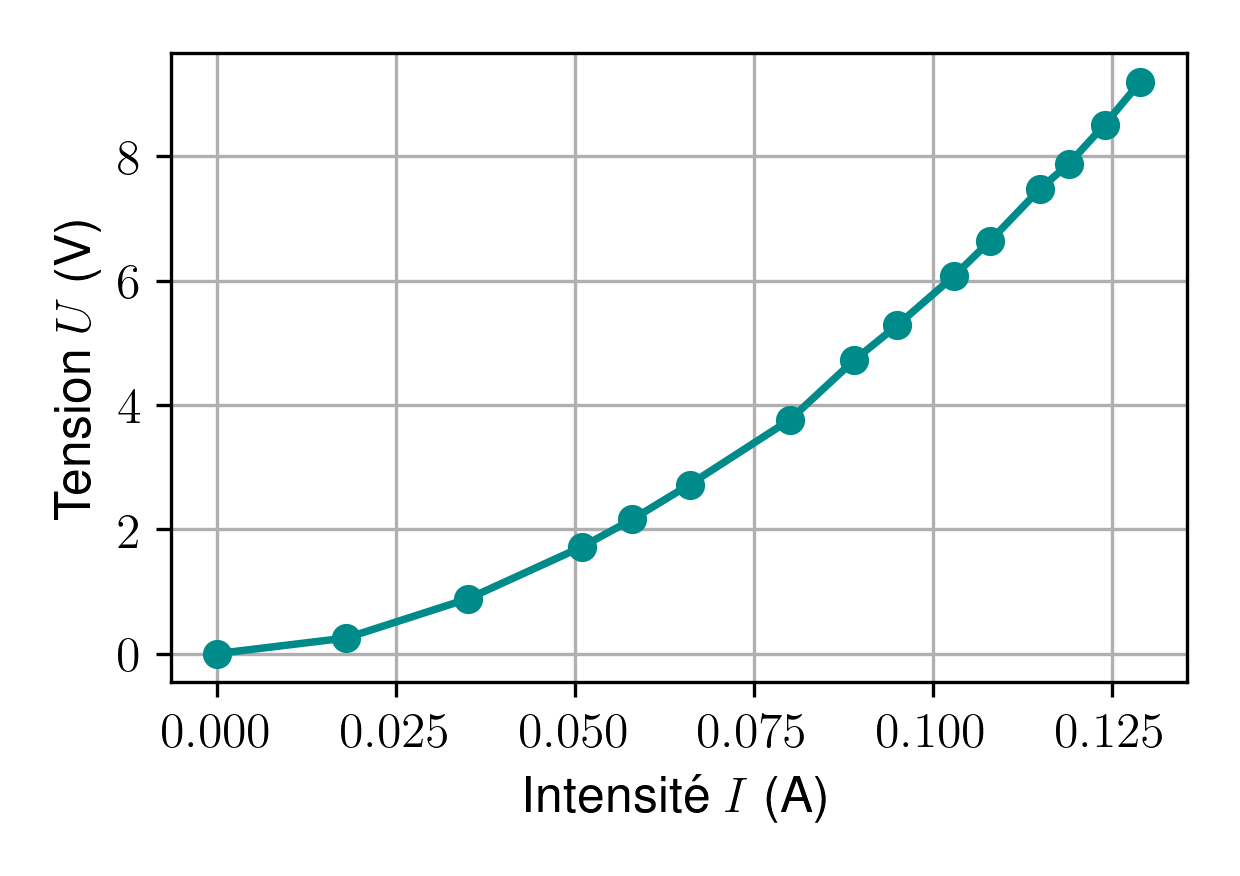
\includegraphics[width=.95\textwidth]{CaracteristiqueLampe.png}
\end{minipage}\hfill
\begin{minipage}{.35\textwidth}
	La courbe caractéristique d'une lampe à incandescence n'est pas une droite passant par l'origine comme pour la résistance.
\end{minipage}
\subsubsection{Le générateur de tension continue}
Un générateur de tension à la particularité de posséder une tension à ses bornes lorsqu'il est isolé sans circuit extérieur, c'est à dire en l'absence de courant. 

\begin{minipage}{.5\textwidth}
	\centering
	\includegraphics[width=.95\textwidth]{CaractéristiqueGenerateur.png}
\end{minipage}\hfill
\begin{minipage}{.4\textwidth}
	Lorsqu'une pile délivre du courant, la tension à ses bornes diminue progressivement. La caractéristique est pratiquement une droite d'équation :

	\begin{equation}
		U = E-rI
	\end{equation}
	E est la tension à vide de la pile, $r$ est une resistance interne de la pile. Donc la caractéristique $U=f(I)$ est une droite. 
\end{minipage}
\clearpage
\subsection{Point de fonctionnement}

Lorsqu'un dipôle récepteur est branché aux bornes d'un générateur, un courant de même intensité $I_f$, traverse les deux dipôles. La tension $U_f$ à leur bornes est également la même. ces deux conditions sont réalisées simultanément à l'intersection des caractéristiques des deux dipôles. 

\begin{figure}[ht]
	\centering
	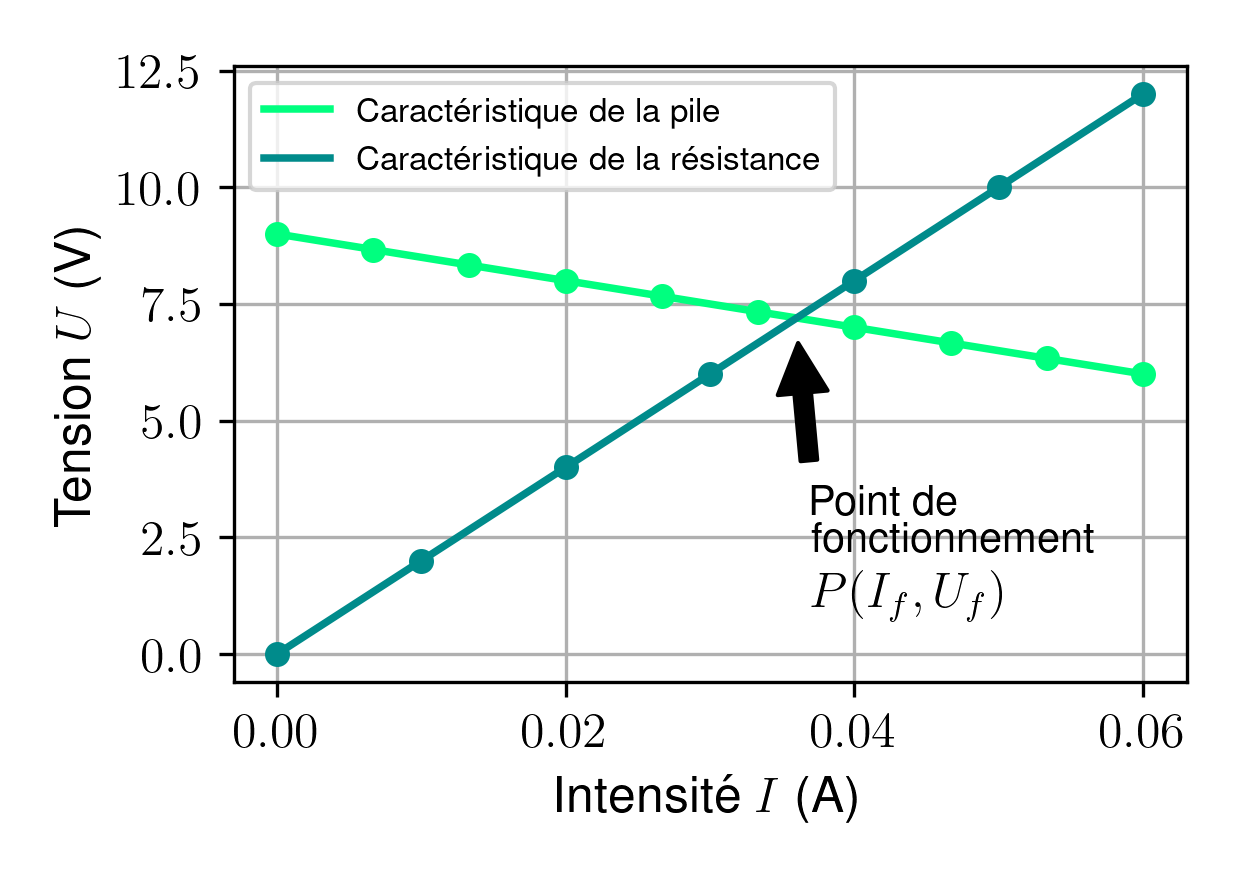
\includegraphics[width=.6\textwidth]{PointDeFonctionnement.png}
	\caption{Point de fonctionnement d'un circuit composé d'un générateur et d'un conducteur ohmique.}
\end{figure}

\begin{definition}{Définition 7 - Le point de fonctionnement d'un dipôle}

	Le point de fonctionnement d'un circuit est noté $P(I_f; U_f)$. C'est le point d'intersection des caractéristiques du générateur et du dipôle recepteur branché sur le générateur. 

\end{definition}

\section{Les capteurs}

On utilise tous les jours parfois sans s'en rendre compte des capteurs. En effet les capteurs sont présents dans de nombreux appareils mécaniques et électroniques comme dans les voitures, les téléphones ou bien les montres connectées.\medskip

\begin{definition}{Définition 8 - les capteurs}

	Un capteur est un dispositif permettant de capter un phénomène physique et de le restituer sous forme de signal électrique. 
	
\end{definition}

\doc{3}{Capteur}{
	\centering
	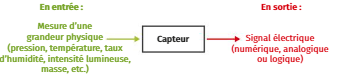
\includegraphics[width=.7\textwidth]{capteur.png}
}

\subsection{Les capteurs dans votre smartphone} 

Certains dipôles sont couramment utilisés comme capteurs : la photorésistance (capte l'éclairement), la thermistance (pour la température), les capteurs de mouvements (pour l'accélération), le capteur de champ magnétique ou encore de pression. Tous ces capteurs se trouvent dans votre smartphone aujourd'hui ce qui vous permet de jouer à des jeux vidéos mais ils en font un outil pour faire de la physique très puissant ! 

\subsection{Activité : à la découverte des capteurs de votre smartphone}

\subsubsection{Découverte des capteurs }

\doc{1}{L'application Phyphox sur Android et IOS}{

Avant de pouvoir vous lancer sur les défis qui vont être proposé ci-dessous il vous faudra installer l'application \textit{phyphox sur votre smartphone}\smallskip

\centering
	\begin{minipage}{.3\textwidth}
		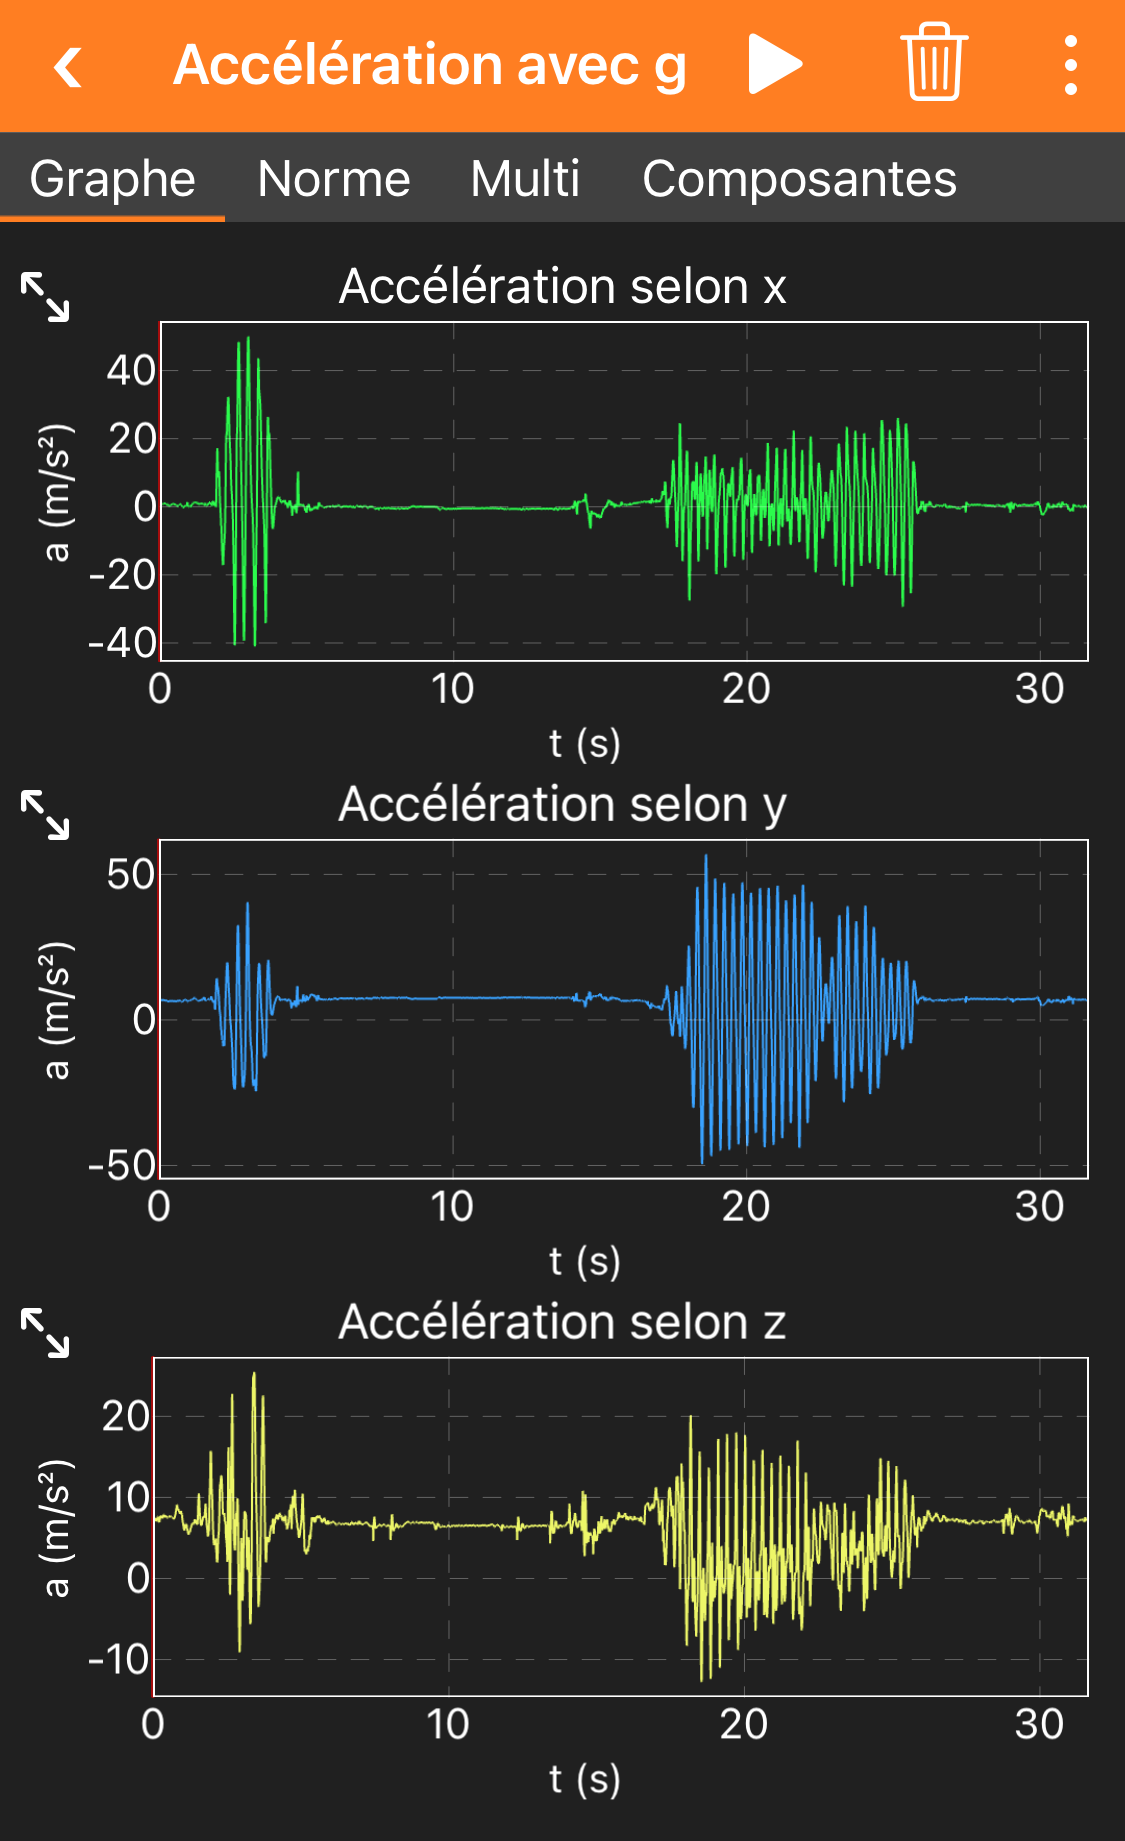
\includegraphics[width=1\textwidth]{Phyphox.png}
	\end{minipage}\hspace{2cm}
	\begin{minipage}{.3\textwidth}
		
\includegraphics[width=1\textwidth]{PhyphoxQRcode.png}
	\end{minipage}\smallskip

	\textbf{\textit{À gauche mesure de l'accélération à l'aide de l'application. À droite le lien vers le site web de Phyphox pour télécharger l'application.}}

}

% \doc{2}{Découvrir les capteurs présents dans votre smartphone}{

% Vous pouvez découvrir comment fonctionnent les différents capteurs présents dans votre smartphone en allant sur la page suivante : \footnote{\url{https://hebergement.universite-paris-saclay.fr/supraconductivite/projet/les_capteurs_dans_un_smartphone/}}{\href{https://hebergement.universite-paris-saclay.fr/supraconductivite/projet/les_capteurs_dans_un_smartphone/}{\textcolor{blue}{Cliquez ici pour accéder à la documentation}}, 
% }


\subsubsection{Mesurer avec votre smartphone des phénomènes Physique}

	Nous allons mettre à l'épreuve les capteurs de votre smartphone en l'utilisant pour faire de la physique. Le smartphone contient différents capteurs. Je vous propose d'en utiliser 3 mais vous êtes libre d'en utiliser d'autres. Vous trouverez la liste des capteurs présents dans le smartphone ici : \url{https://hebergement.universite-paris-saclay.fr/supraconductivite/projet/les_capteurs_dans_un_smartphone/}.\medskip

	Sur la page suivante, je vous propose d'étudier trois capteurs le microphone, le gyroscope et le magnétomètre. Et enfin de réaliser 8 petits défis à l'aide de vos capteurs de smartphone \url{https://gledoudic-drive.mytoutatice.cloud/public?sharecode=ZkYBED84BEOS}\medskip

	Si vous avez besoin d'explication des petites vidéos sont là pour expliquer le fonctionnement des capteurs sur ce lien \footnote{\url{https://hebergement.universite-paris-saclay.fr/supraconductivite/projet/les_capteurs_dans_un_smartphone/}}
	
\clearpage

\doc{3}{Mesurer la période, la fréquence et le niveau d'intensité de votre voix}{
\centering
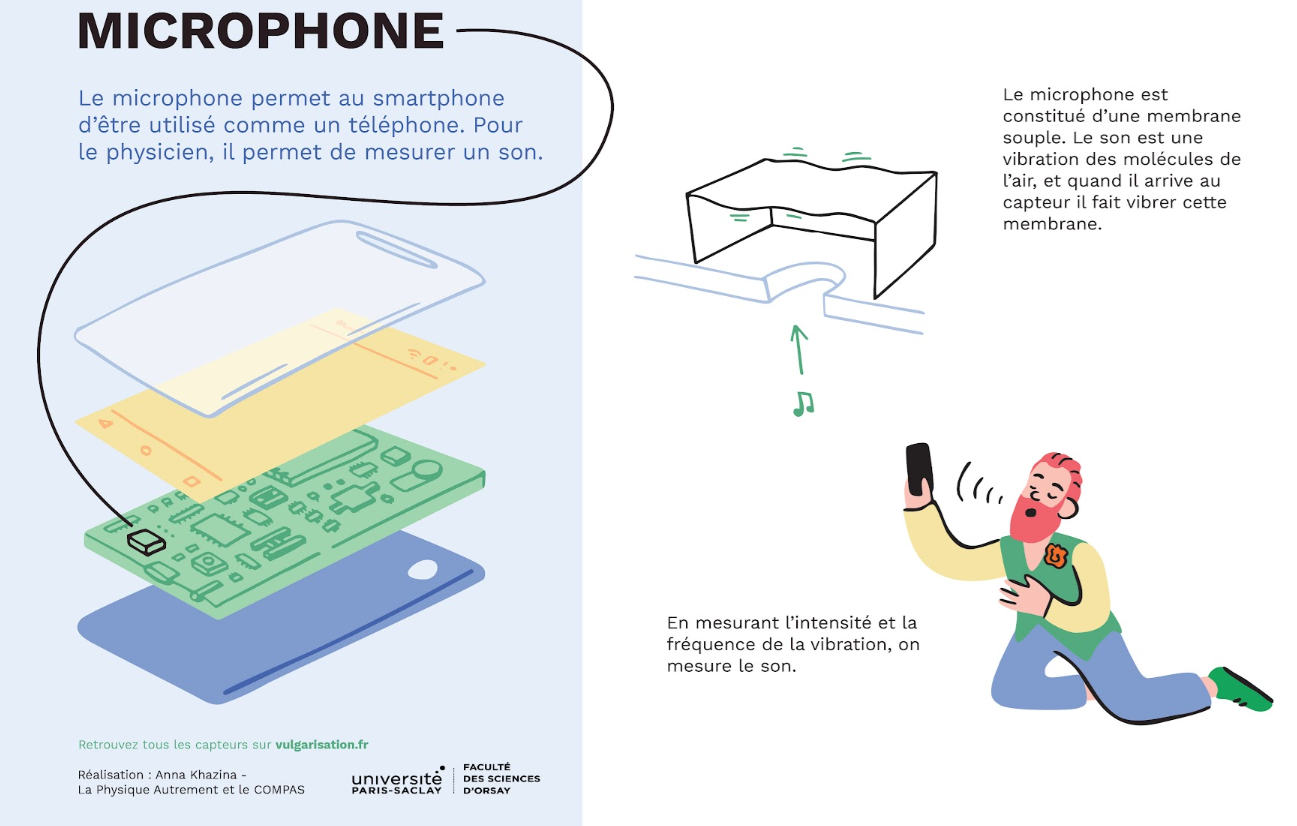
\includegraphics[width=.6\textwidth]{Microphone.png}
}

\doc{4}{Détecter et mesurer le mouvement et l'accélération}{
\centering
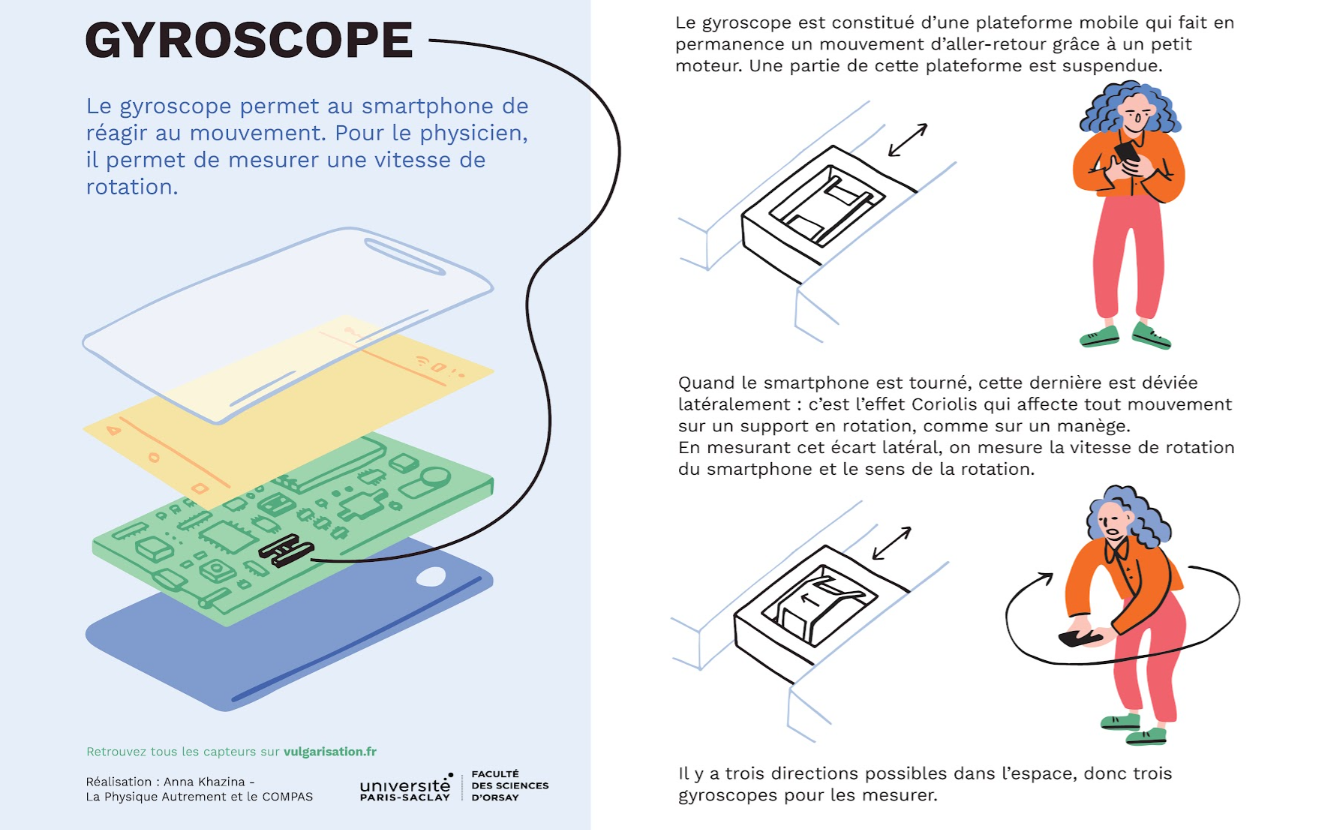
\includegraphics[width=.6\textwidth]{Gyroscope.png}
}

\doc{5}{Mesurer le champ magnétique de la Terre}{
	\centering
	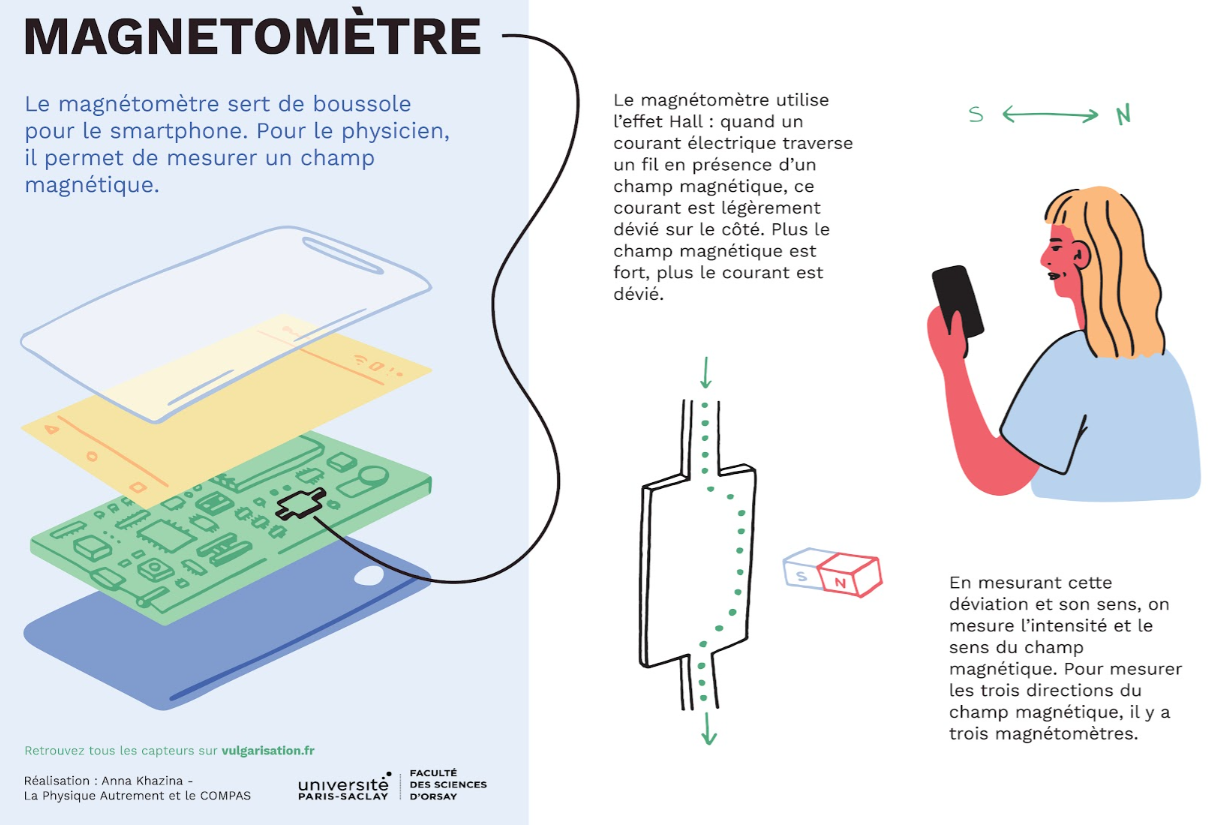
\includegraphics[width=.6\textwidth]{Magnetometre.png}
}

\end{document}

%%
%% FIN DU DOCUMENT
%%
